\chapter{Architektur}
Im folgenden Abschnitt wird die Architektur der Applikation diskutiert. Die Architektur ist so gewählt, dass die einzelnen funktionalen Komponenten zueinander eine tiefe Abhängigkeit aufweisen und dadurch eine weitere Entwicklung möglichst einfach ist.

\section{Klassendiagramm}
Die Domainlogik beinhaltet die Kernelemente der Applikation. Einerseits sind dies die Rennfahrer, welche Informationen über sich festhalten andererseits die Etappe mit den Informationen zur Strecke. Während dem Rennen werden die Fahrer in Gruppen unterteilt. Auch diese Gruppen sind in der Domain abgebildet. Das Klassendiagramm des Domain Package zeigt die wesentlichen Elemente.

\begin{figure}[h!]
\caption{Die Domainklassen in der Abhängigkeit}
\label{fig:domain}
\centering
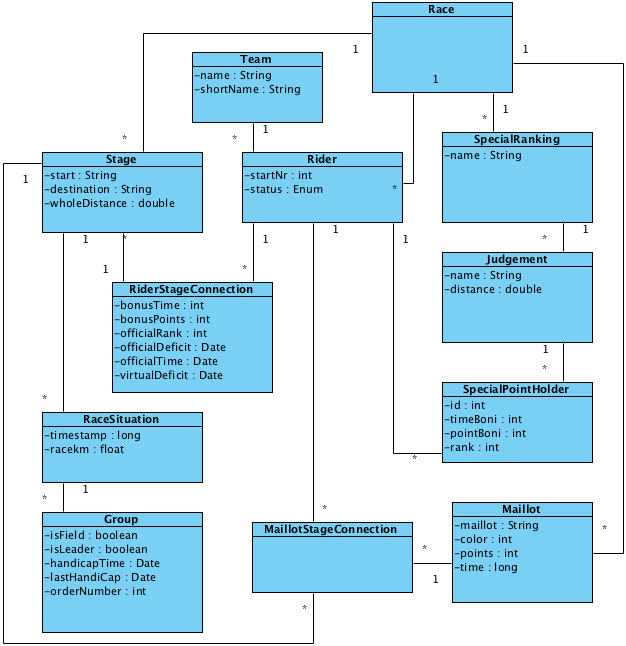
\includegraphics{05bericht/images/domain.png}
\end{figure} 


\textit{Rider} speichert die Angaben zu einem Fahrer und beinhaltet keine eigene Logik. Ein Fahrer hat immer genau ein \textit{RiderState}. Dies ist ein Java \gls{enum} und zeigt den Status des Fahrer an. Nach dem Import der Fahrerliste werden alle Fahrer auf \textit{activ} gesetzt.
\\
In \textit{Stage} ist die Etappe definiert. Jede Etappe hat eine Marschtabelle in Form von mehreren \textit{PointOfRace} Objekten. Diese Objekte werden durch Import der Marschtabelle erstellt.
\\
Da pro Etappe jeder \textit{Rider} einen anderen \textit{RiderState} haben kann, gibt es die Verbindungsklasse \textit{RiderStageConnection}. In dieser Klasse ist jeweils die Etappe mit dem Fahrer verknüpft. Dies ermöglicht es den Rückstand eines Fahrers in mehreren Etappen zu verfolgen.
Ein \textit{Judgement}, also eine Wertung, gehört immer zu einer Etappe. Diese Wertungen sind definiert durch ein \textit{SpecialRanking}, welche Punkte- und Zeitboni beinhalten können.

\section{Sequenz Diagramm}
Der häufigste UseCase besteht darin, die Rennsituation zu erfassen und an den Server zu übermitteln. Gleichzeitig werden im Hintergrund die Live Informationen aktualisiert. Diese beiden Hauptanwendungsfälle sind im folgenden System Sequenz Diagramm dargestellt. Der Aktor wird durch den \textit{RadioTour Speaker} dargestellt und das System durch die \textit{RadioTour} Applikation. Das externe System stellt die Serverseite dar.

\begin{figure}[h!]
\caption{Das System Sequenz Diagramm}
\label{fig:domain}
\centering
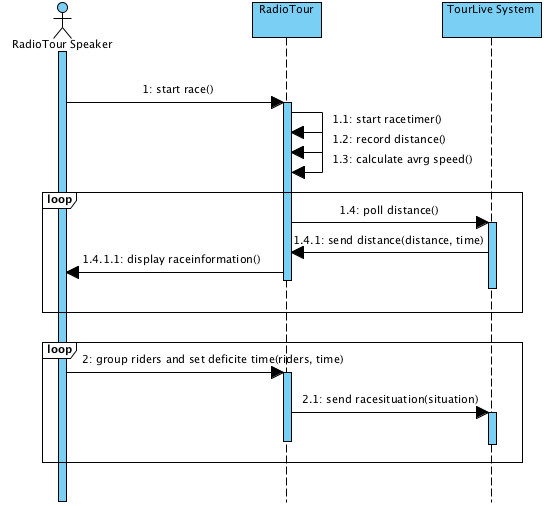
\includegraphics{05bericht/images/ssd_rennen.png}
\end{figure} 

Das Rennen wird durch das Starten der Rennzeit gestartet. Ab diesem Zeitpunkt beginnt die Aufzeichnung des Rennkilometers und die Berechnung der durchschnittlichen Geschwindigkeit.